%\documentstyle[10pt,twoside]{article}
%\documentstyle[twoside]{article}
\documentclass[twoside]{article}
\setlength{\oddsidemargin}{0.25 in}
\setlength{\evensidemargin}{-0.25 in}
\setlength{\topmargin}{-0.6 in}
\setlength{\textwidth}{6.5 in}
\setlength{\textheight}{8.5 in}
\setlength{\headsep}{0.75 in}
\setlength{\parindent}{0 in}
\setlength{\parskip}{0.1 in}

\usepackage{graphicx}
\usepackage{url}

%
% The following commands sets up the lecnum (lecture number)
% counter and make various numbering schemes work relative
% to the lecture number.
%
\newcounter{lecnum}
\renewcommand{\thepage}{\thelecnum-\arabic{page}}
\renewcommand{\thesection}{\thelecnum.\arabic{section}}
\renewcommand{\theequation}{\thelecnum.\arabic{equation}}
\renewcommand{\thefigure}{\thelecnum.\arabic{figure}}
\renewcommand{\thetable}{\thelecnum.\arabic{table}}
\newcommand{\dnl}{\mbox{}\par}

%
% The following macro is used to generate the header.
%
\newcommand{\lecture}[4]{
   \pagestyle{myheadings}
   \thispagestyle{plain}
   \newpage
   \setcounter{lecnum}{#1}
   \setcounter{page}{1}
   \noindent
   \begin{center}
   \framebox{
      \vbox{\vspace{2mm}
    \hbox to 6.28in { {\bf CMPSCI~677~~Distributed Operating Systems
                        \hfill Spring 2019} }
       \vspace{4mm}
       \hbox to 6.28in { {\Large \hfill Lecture #1: #2  \hfill} }
       \vspace{2mm}
       \hbox to 6.28in { {\it Lecturer: #3 \hfill Scribe: #4} }
      \vspace{2mm}}
   }
   \end{center}
   \markboth{Lecture #1: #2}{Lecture #1: #2}
   \vspace*{4mm}
}

%
% Convention for citations is authors' initials followed by the year.
% For example, to cite a paper by Leighton and Maggs you would type
% \cite{LM89}, and to cite a paper by Strassen you would type \cite{S69}.
% (To avoid bibliography problems, for now we redefine the \cite command.)
%
\renewcommand{\cite}[1]{[#1]}

% \input{epsf}

%Use this command for a figure; it puts a figure in wherever you want it.
%usage: \fig{NUMBER}{FIGURE-SIZE}{CAPTION}{FILENAME}
\newcommand{\fig}[4]{
            %\vspace{0.2 in}
            \centerline{\includegraphics[scale=#2]{#4}}
            \begin{center}
            Figure \thelecnum.#1:~#3
            \end{center}
    }

% Use these for theorems, lemmas, proofs, etc.
\newtheorem{theorem}{Theorem}[lecnum]
\newtheorem{lemma}[theorem]{Lemma}
\newtheorem{proposition}[theorem]{Proposition}
\newtheorem{claim}[theorem]{Claim}
\newtheorem{corollary}[theorem]{Corollary}
\newtheorem{definition}[theorem]{Definition}
\newenvironment{proof}{{\bf Proof:}}{\hfill\rule{2mm}{2mm}}

% Some useful equation alignment commands, borrowed from TeX
\makeatletter
\def\eqalign#1{\,\vcenter{\openup\jot\m@th
  \ialign{\strut\hfil$\displaystyle{##}$&$\displaystyle{{}##}$\hfil
      \crcr#1\crcr}}\,}
\def\eqalignno#1{\displ@y \tabskip\@centering
  \halign to\displaywidth{\hfil$\displaystyle{##}$\tabskip\z@skip
    &$\displaystyle{{}##}$\hfil\tabskip\@centering
    &\llap{$##$}\tabskip\z@skip\crcr
    #1\crcr}}
\def\leqalignno#1{\displ@y \tabskip\@centering
  \halign to\displaywidth{\hfil$\displaystyle{##}$\tabskip\z@skip
    &$\displaystyle{{}##}$\hfil\tabskip\@centering
    &\kern-\displaywidth\rlap{$##$}\tabskip\displaywidth\crcr
    #1\crcr}}
\makeatother

% **** IF YOU WANT TO DEFINE ADDITIONAL MACROS FOR YOURSELF, PUT THEM HERE:



% Some general latex examples and examples making use of the
% macros follow.

\begin{document}

%FILL IN THE RIGHT INFO.
%\lecture{**LECTURE-NUMBER**}{**DATE**}{**LECTURER**}{**SCRIBE**}
\lecture{19}{April 17}{Prashant Shenoy}{\textbf{Mikayla Timm}}

In this lecture, professor wraps up the discussion of fault tolerance and starts a new topic ``World Wide Web", as the topic helps in getting started with Lab 3.
\section{Raft Consensus Protocol}
Paxos is very hard to reason about. Therefore, another consensus protocol Raft is developed with an aim to make it easier to understand. It is not meant to perform everything that Paxos does, but it works in the presence of failures. In Paxos, we had to agree on operations like state of lock, order of applying queries etc. Raft is specially designed for replicated servers, where all of the servers process the same request. When a request comes in, the request is forwarded to all the replicas, so that all of them could perform the same action and be consistent. When multiple requests come in, we have to order them and send them in the same order to all the replicas. \\
Raft uses a technique called State Machine Replication(SMR), which became popular in distributed systems. SMR maintains a log file in each replica. This log is used to determine the order in which the requests come in. Requests are written to the logs in the same order, so the logs at all of the replicas will be the same. If we perform the operations in same order for all replicas, then they will be consistent.\\
Raft is not completely distributed. First a leader is elected and this leader decides an ordering and imposes the ordering on all the followers. If the majority agrees on the ordering, the ordering is committed and minority which does not agree will have to synchronize at a later time before they can execute requests.\\

\textbf{Question:} Without using Raft, how do we ensure database consistency?\\
\textbf{Answer:} Can have frontend node send the same request to all replicas, or have a master node that receives all requests and sends it to where it needs to go in a single order.\\
\begin{figure}[h]
\begin{center}
\fbox{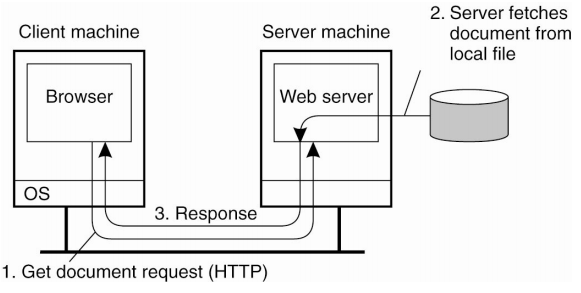
\includegraphics[scale=0.4]{traditional_web_based.png}}
\caption{Overall Organization of a Traditional Web Site}
\label{traditional_web_based}
\end{center}
\end{figure}
\section{Traditional Web Based Systems}
Figure \ref{traditional_web_based} shows a basic client-server request response protocol. Browser sends a HTTP request to the web server. The server fetches the document from database and sends back the response to the browser.
\section{Processes - Clients}
\begin{figure}[h]
\begin{center}
\fbox{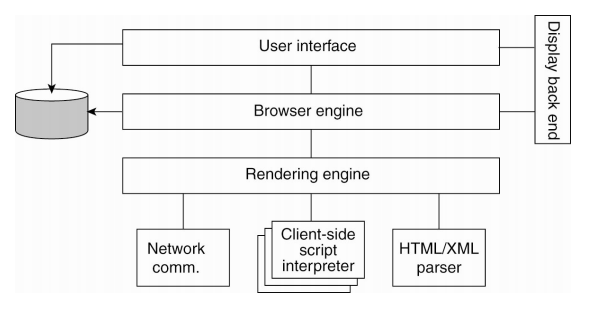
\includegraphics[scale=0.4]{process_client1.png}}
\caption{Logical Components of a Web browser}
\label{components}
\end{center}
\end{figure}
Browsers are complex with many built-in functionalities. Figure \ref{components} shows the major components of a web browser. The rendering engine takes a HTML documents and renders it on the user screen. The Client side interpreter interprets the Java/PHP scripts embedded in the documents. \\
Proxy is an entity which lies between the client and the server. They are commonly used for web caching. Recently used web pages are cached. The browser will send requests to the proxy instead of server. Proxy will process the request. If the requested content is cached on proxy, it is will send back reply to client. Else, the proxy makes another request to the server.\\
\begin{figure}[h]
\begin{center}
\fbox{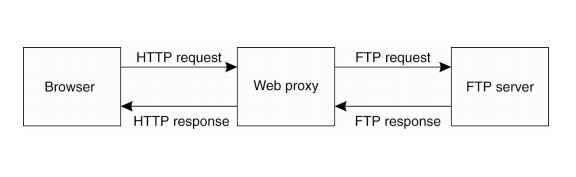
\includegraphics[scale=0.4]{transcoding.png}}
\caption{Web Proxy for Transcoding}
\label{transcoding}
\end{center}
\end{figure}
Proxies can also be used for transcoding. Transcoding refers to actively changing content to better cater user needs. For example, adjusting the web page layout to make it suitable for mobile display. The example shown in figure \ref{transcoding} does protocol translation. Another example is rendering video content - the proxy may translate high definition video to standard definition.

\section{Apache Web Server}
\begin{figure}[h]
\begin{center}
\fbox{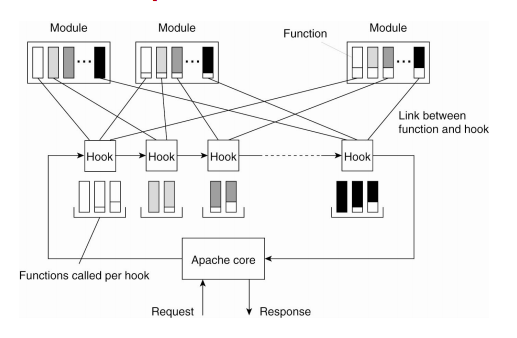
\includegraphics[scale=0.4]{apache_server.png}}
\caption{Overall Organization of Apache Web Server}
\label{apache_web}
\end{center}
\end{figure}
Figure \ref{apache_web} is a Apache Web Server. It has a modular architecture. We need to configure a set of modules that will perform request processing. When a request comes in, it will go through a series of processing steps. Each module performs partial processing in a pipeline fashion. You can turn each module on or off.\\

\textbf{Question:} What is an example for pipeline processing?\\
\textbf{Answer:} Let's say the client has sent an HTTPS request, which means the connection is encrypted. First, one of modules decrypts the request. The next module extracts the web pages. The PHP commands in the web page are processed using an interpreter module. At the end, a module have to encrypt the response. These are some sequence of steps. \\
This server can also have multi-tier architecture. We can employ caching at multiple levels of these tiers. For example, database queries can be cached. 
\section{Web Server Clusters}
\begin{figure}[h]
\begin{center}
\fbox{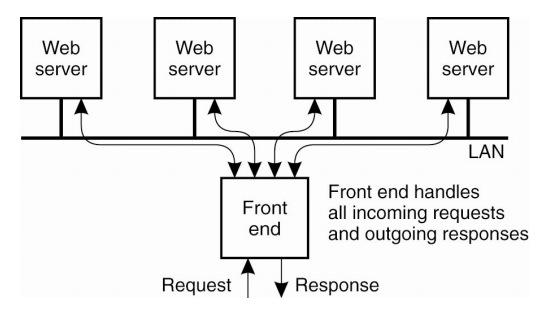
\includegraphics[scale=0.4]{clusters_1.png}}
\caption{Web Server Clusters}
\label{cluster_1}
\end{center}
\end{figure}
Figure \ref{cluster_1} shows an example of clustered architecture. Each box are themselves multi-tiered. Each incoming request can be forwarded to one of the four Web Servers. Responses flow back through the load balancing switch. The clusters can service more requests, which allows it to scale up better.\\
\begin{figure}[h]
\begin{center}
\fbox{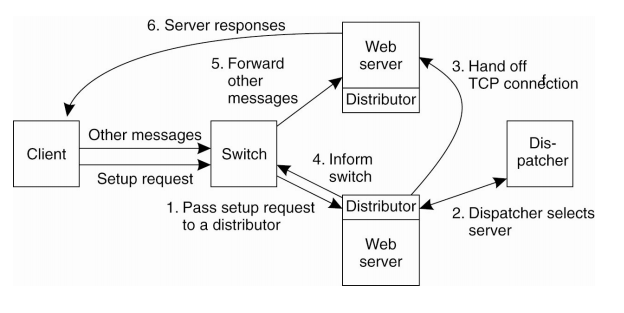
\includegraphics[scale=0.4]{cluster_2.png}}
\caption{Scalable Content-Aware Cluster of Web servers}
\label{cluster_2}
\end{center}
\end{figure}
Figure \ref{cluster_2} depicts another such architecture. The dispatcher is responsible for balancing the load. Each client is mapped to one of the servers. Once mapped, the switch will store this information and uses it to forward all consecutive requests from that client to the mapped server.\\\\
\textbf{Question:} Why is the dispatcher not dispatching the messages?\\
\textbf{Answer:} There can be many different architectures. The specific example shown here is doing session level dispatching. This means that every user is mapped once to a web server. From that point, the requests from that browser will be sent to the same server without further need of dispatching.\\\\
\textbf{Question:} Can the switch be a bottleneck?\\
\textbf{Answer:}If we have high volume of requests, the switch could become a bottleneck. It is simply forwarding the request. We can make it distributed as well. If we are not doing much processing and if implemented in hardware, it can support high request rate.\\\\
\textbf{Question:} When the session begins, do you talk to the dispatcher?\\
\textbf{Answer:} Yes. We typically go from a web server to the dispatcher. Dispatcher selects the server. It informs to the switch. And from that point switch takes over.
\section{HTTP Connections}
\begin{figure}[h]
\begin{center}
\fbox{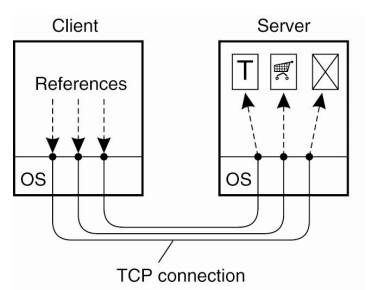
\includegraphics[scale=0.4]{http_1_0.png}}
\caption{HTTP 1.0: Using Non-Persistent Connections.}
\label{http_1.0}
\end{center}
\end{figure}
Figure \ref{http_1.0} shows the original HTTP 1.0, where browser sets up a new TCP connection to the server every time we make a HTTP request. The connection is then set down. If there are hyper links, it will create new connection. Making new connection to the same server every time is wasteful. A variant, version 1.1 Persistent HTTP from figure \ref{http_1.1} uses a single connection and piggy backs requests. The browsers does not close the connection immediately, in anticipation of further requests. This reduces the overhead to the server, as it limits the number of socket connections.\\\\
\begin{figure}[h]
\begin{center}
\fbox{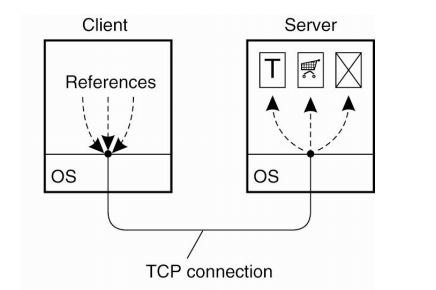
\includegraphics[scale=0.4]{http_1_1.png}}
\caption{HTTP 1.1: Using Persistent Connections.}
\label{http_1.1}
\end{center}
\end{figure}
\textbf{Question:} This has to enabled on the server side?\\
\textbf{Answer:} Yes. If the server can support HTTP 1.1 then we can use it. The first time when browser sends a request to the server, it asks for the version of HTTP. \\

\textbf{Question:} How does the client browser differentiate between the two types of dispatcher? \\
\textbf{Answer:} The client browser should not even know about the presence of dispatcher. \\
One of the design issues for HTTP 1.1 is the duration of time to keep the connection open. Should the browser wait for 5min or 1hr? This is a design decision. As server will receive requests from multiple other users, this problem is even worse because of open socket connections. Usually, server closes the connection, if the connection is ideal for long time.
\section{HTTP Methods}
HTTP protocol has five commands:
\begin{enumerate}
    \item The simplest among them is the 'GET' command. This command allows the user to request and get a document.
    \item While 'PUT' command is used to send the document to the server. 'PUT' is only used if the server have WebDev service.
    \item 'POST' is the most common command. It allows the user to send information back to the server.
    \item 'DELETE' can be used to delete a page on server.
    \item 'HEAD' gets the header of the document. It is typically used for caching.
\end{enumerate}  

\textbf{Question:} Which command can be used to update information on the server?\\
\textbf{Answer:} First, do a 'GET' to get the web page with form embedded in it, once you fill the form and submit it will go as a  'POST' request. \\

\section{Web Services Fundamentals}
\begin{figure}[h]
\begin{center}
\fbox{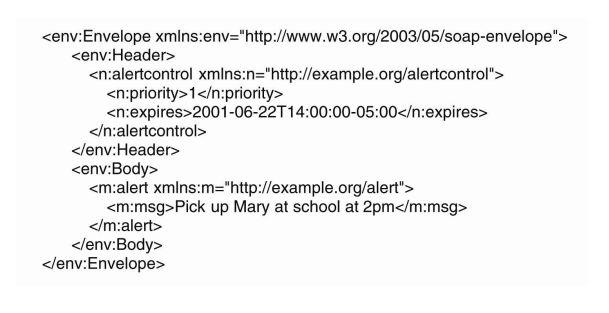
\includegraphics[scale=0.5]{soap_xml.png}}
\caption{Example of XML-based SOAP message}
\label{soap_ex}
\end{center}
\end{figure}
HTTP is not only confined to typical interactions between users through browsers. It also facilitates process to process communication. In this case, the two applications communicate without human interaction. RPC is an example of such communication. SOAP (Simple Object Access Protocol) was initial protocol used to make RPC request over HTTP. The entire RPC request is sent as a XML document. The server after receiving the document, parses it, perform required operation and sends back the response as another XML document. Figure \ref{soap_ex} shows one such XML request document. Here the client is calling 'alert' method and passing the string 'Pick up Mary at school at 2pm' as an argument to that method. \\

\section{Restful Web Services}
As we can see, for calling single method with one argument, we have to send such a long XML file. SOAP did not perform well because of this overhead. As a result, SOAP evolved into Restful architecture. Restful architecture also makes RPC request over HTTP. In case of Restful architectures, the communication is light weight and assumes one-to-one communication between client and server. \\
\begin{figure}[h]
\begin{center}
\fbox{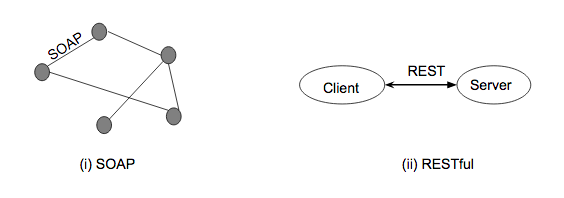
\includegraphics[scale=0.5]{inclass-diag.png}}
\caption{SOAP vs RESTful Connections}
\label{soap_rest}
\end{center}
\end{figure}
\textbf{Question:} What do you mean by saying 'SOAP requires arbitrary servers'?\\
\textbf{Answer:} SOAP is designed for an arbitrary distributed application, where there are arbitrary number of nodes, that are all communicating over RPC to implement a larger application. Each edge connecting the nodes in figure \ref{soap_rest} (i) is a SOAP interface. So, SOAP is designed for general distributed application scenarios. On the other hand, Restful web services(\ref{soap_rest} (ii)) assume one client is talking to only one server through HTTP based REST requests. We assume there is no state. It will simplify a lot of things. \\

In the case of RPC requests, Restful services will send the method name and arguments in the URL itself, as opposed to sending a complex XML document as we did in the case of SOAP. \\
\textbf{Question:} How do you send string where there is a space in them in the request URL?\\
\textbf{Answer:} You will use control characters to describe it. For example, "IBM Research" can be encoded as "IBM\%20Research". It depends on the HTTP specification.\\
\textbf{Question:} Is there any limit on the length of the characters?\\
\textbf{Answer:} There should not be any such constraints.\\\\
\textbf{Question:} Why is the XML document a problem in the case of SOAP?\\
\textbf{Answer:} Parsing the XML document is a processing overhead. It effects efficiency. In the case of Restful architecture processing overhead is minimized as the method name and parameters are part of URL.\\

\section{SOAP VS RESTful WS}
\begin{enumerate}
    \item SOAP application can be written in various languages and can run on different platforms. It need not use HTTP. Whereas, RESTful services only support HTTP.
    \item SOAP supports arbitrary set of inter-communicating applications. Where as REST uses point to point connection with no intermediaries. 
    \item SOAP has a wide set of standard, whereas RESTful services does not have any pre-defined standards
    \item Over head is higher with SOAP compared to REST.
    \item Rest has less of a learning curve compared to SOAP.
\end{enumerate}

\section{Web Proxy Caching}
The discussion for this section assumes a collection of proxy caches sitting in between the client and the server. Along with communicating with the server, these proxy caches can also communicate with each other. This mechanism is called ``Cooperative Caching". Figure \ref{coop_cache} shows one such scenario where a client sends a request to the web proxy. The web proxy will then look into it's local cache for the requested web page. If it is a hit, then it will send the response back. In the case of miss, typically the web proxy will contact server. But in the case of cooperative caching, it will reach out to the near by proxies to get the data. This can make fetching faster. The cache becomes the union of all caches.
\begin{figure}[h]
\begin{center}
\fbox{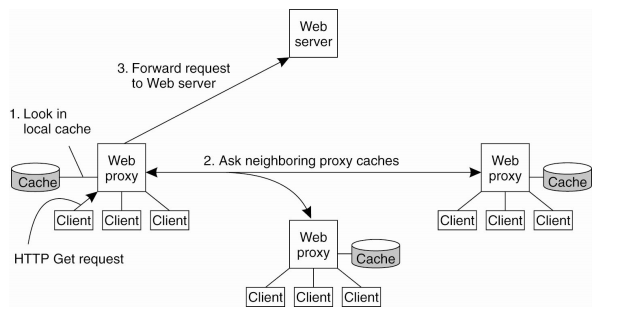
\includegraphics[scale=0.5]{coop_caching.png}}
\caption{Cooperative Caching}
\label{coop_cache}
\end{center}
\end{figure}
\section{Web Caching}
It is also import to deal with consistency. Web pages tend to change with time. When a browser fetches a page from the server, we are guaranteed that the returned page is the most recent version. While using proxies, we need to ensure the consistency of cache web pages. The popularity and update frequency can be different across web pages. We need to consider both these issues for maintaining consistency. We need to make sure the caches have the most new/updated version. There are different methods for this:

\begin{enumerate}
    \item Client Pull VS Server Push
    \item Invalidate VS update: 
        \subitem \textbf{Invalidate}: server just notifies the proxy that web page has changed. The proxy will then remove the page entry from it's cache. 
        \subitem \textbf{Update}: server actually sends the updated page to the proxy. 
\end{enumerate}

\subsection{Push-based Approach}
In this approach, the web server will keep track of web pages requested by every proxy so that it knows which proxies cached each page. Whenever a web page is changed, the server will either a notification(invalidate) or the new version(update) to the set of proxies which cached this page. If the web page is popular it makes more sense to send updated version to the proxy. Else, if it is less popular, it makes more sense to send an invalidate. Push-based approach provides tight consistency guarantees. Proxies can also be passive, as the server does all the work in this approach. One disadvantage is that, since HTTP is stateless, you need mechanisms beyond HTTP. Another disadvantage is that the server needs to keep track of proxies forever.\\\\
\textbf{Question:} What happens in the case of invalidate?\\
\textbf{Answer:} Once the proxy receives invalidate message from the server, it will delete the entry from the cache. Later, when some client requests for that web page, the proxy gets a cache miss. So, the proxy will fetch it from the server.\\\\
\textbf{Question:} Is caching with proxies similar to edge servers?\\
\textbf{Answer:} Proxies can be deployed anywhere in a network. Edge servers put computation specifically at the edge of the network.
\subsection{Pull-based Approach}
Proxy is responsible to maintain consistency. It polls the server periodically to check if the previously cache page has changed. Polling is performed using conditional GET (if-modified-since HTTP messages). That is if the web page has changed since the timestamp 't', GET me the updated web page. For web pages which changes very rarely, frequent pooling is extremely wasteful. There is no such wasteful messages in push based approach. If the page changes much more frequently than polling frequency then the proxy might cached outdated content for longer times. Polling frequency should be decided based on the update frequency of web page. There are two ways to do this:
\begin{enumerate}
    \item Server can assign a expiration time (TTL: time-to-live values). This time is an estimation of next possible changes on the web page. Server can estimate it based on the past web page update frequency history.
    \item Proxy has intelligence to dynamically figure out the polling times. Poll duration is varied based on the observed web page updates. 
\end{enumerate}
Pull based approach gives weaker consistency guarantees. Updates of a web page at server, might not be immediately reflected at proxies. Latency to sync the content might overtake the benefits of proxies. There is a higher overhead than server push approach, and there could be more pulls than updates. Some advantages are that the pull based approach can be implemented using HTTP (server remains stateless). This approach is also resilient to both server and proxy failures.
\section{A Hybrid Approach: Leases}
Lease is a contract between two entities in the distributed system. It specifies the duration of time the server agrees to notify the proxy about any updates on the web page. Updates are no longer sent by the server after lease expiration and the server will delete the state. Proxy can renew the lease. 

\subsection{Policies for Leases Duration}
Lease duration is an important parameter. Zero duration is a pure proxy pull approach which result in increased polling requests. Where as, infinite lease is server-push approach which makes the server stateful. There are three policies for lease duration:
\begin{enumerate}
    \item Age-based: Based on frequency of changes on the object. The age is the time since last update. Assign longer leases for more frequently updated pages.
    \item Renewal-frequency based: Based on frequency of access requests from clients. Popular objects get longer leases.
    \item Server load based: If the load on the server is high, we should use less lease duration. This will remove the burden of storing proxy state on server side.
\end{enumerate}
\begin{figure}[h]
\begin{center}
\fbox{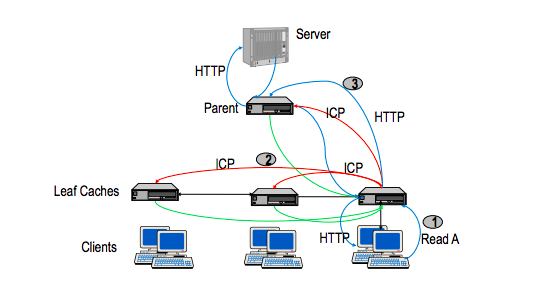
\includegraphics[scale=0.5]{hierarchical_coop.png}}
\caption{Hierarchical Proxy Caching}
\label{hierar_coop}
\end{center}
\end{figure}
\textbf{Question:} In the internet, who owns the proxies? \\
\textbf{Answer:} It depends on the scenario. We can get open source proxy and the user can point the proxy to the browser. Mostly, proxies are run by content distribution networks. They deploy proxy as a service to the end users.\\\\
\textbf{Question:} If the proxy request lease of certain duration, should the server provide it?\\
\textbf{Answer:} There are two options. One option is proxy can request for lease, but server decides the duration. Other option is proxy requesting the duration. First option is better. 
\section{Cooperative Caching}
Figure \ref{hierar_coop} explains the message flow for once single client request in the case of ``Hierarchical Proxy Caching". The client requests for a web page. If it is a cache miss, the proxy will contact it's peers(red arrows). If none of them have it, they will send back the non-availability response to the proxy(green arrows). The proxy will then send an HTTP request to the parent. The parent will fetch the data from the server and sends the web page as response.\\
As we can see, there is a lot of messaging overhead. Also, browser has to wait for longer times in the case of cache miss on the proxy. This will effect performance. Latency could increase - it may have been faster to just directly request from server in the event of a cache miss on the proxy. \\

This is complicated as seen in the figure, as there are many arrows all over the place. To simplify, we can flatten the hierarchy. Keep track of what's cached using table lookup - save which node has what in the table. If there is no entry in the table for a request, go to the server to get it, and add it to the table. Every time you fetch or delete a page, you update the table for all the nodes. Every node keeps a global table that must be kept consistent. All lookups are local. \\

\section{Content Distribution Network}
Companies set up large numbers of caches throughout the world that hold all kinds of content. The DNS figures out which proxy is closest to you.
\end{document}
